% Conduct a motivating experiment that explains
%     Why is this problem important
%     Assuming caches are always good
%         Why multi tier
%         Why partitioning
%             Consider ~10-100 VMs on a single host
%             Global cache is not efficient

\section{Motivation}
The motivation for this work are two-fold. First, we show why we need a smart partitioning algorithm. Second, we show why we need a two-layer cache.

\subsection{The case for smart partitioning}

\begin{figure}[tb]
\setlength{\belowcaptionskip}{-15pt}
\centering
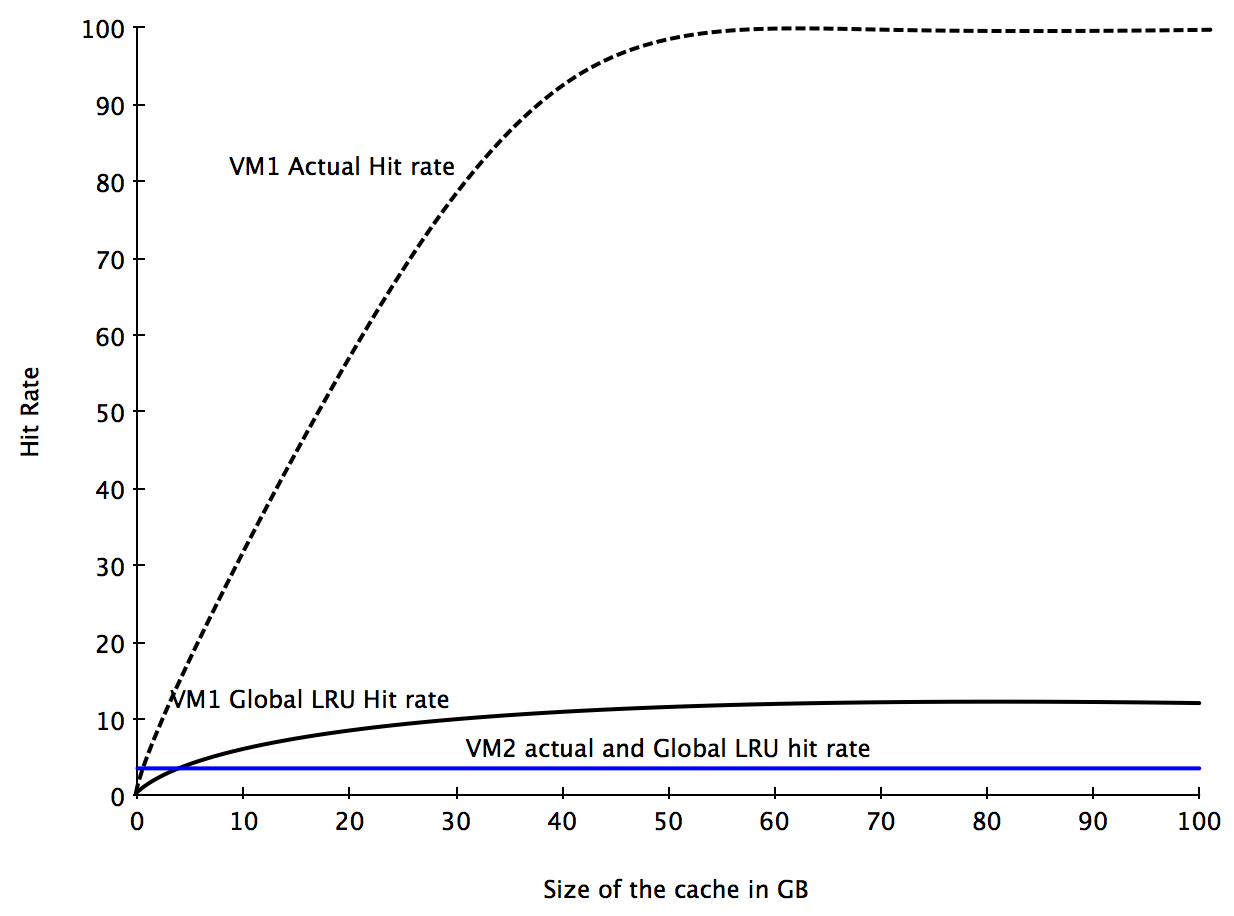
\includegraphics[width=3in]{figures/hitrate_fake}
\caption{VMs competing for resources}
\label{fig:compete}
\end{figure}

The need for partitioning the SSD cache has been studied in [vCacheShare, ...]. To illustrate we conduct a simple experiment where two VMs, namely VM1 and VM2, residing in the same host share a caching device. From figure XX, one can see that VM1 has a high random I/O with a very low hit ratio while VM2 has a low I/O but has a high hit rate. Figure~\ref{fig:compete} , shows that despite VM2 could benefit largely from a cache, it has a very low space allocation in the cache, due to contention from VM1. From figure XX and YY, one can infer that contention can make a cache entirely unusable.

\subsection{The case for two-layer cache}

An ideal solid-state NVM provides fast random-read and random-write accesses. SSD's prices have dropped significantly over the last decade, though they are still expensive compared to disk drives. So, bearing cost vs. performance tradeoffs in mind, it is essential to choose the right caching device to get the maximum performance. Although, much of it depends on the workload of the VMs in the host, one could optimize the cache \note{make a case for using two layers, instead of one}

\begin{center}
  \begin{tabular}{ | l | l | l | }
    \hline
    \textbf{Storage Device} & \textbf{\$/GB} & \textbf{Normalized Price} \\ \hline
    SSD PCIe & 0.9 & 12.65 \\ \hline
    SSD SATA & 0.377 & 5.27 \\ \hline
    HDD & 0.07 & 1 \\
    \hline
  \end{tabular}
\end{center}


As we can see from the figure, there are a number of devices that can be adopted to use as a cache. However the widespread adoption of these devices have always remained slow, mainly because of the difficulty to determine the combination of devices the will give the maximum performance with minimal cost. Another major pain point to utilize these devices efficiently; a bad partitioning strategy would degrade the performance otherwise. The optimization is complex due to the wide variety of devices as well as the workloads in the datacenter.

To overcome these challenges, we propose a dynamically scaling algorithm that not only seamlessly scales to multi-tier caches, but also optimize the caching space for both maximum utilization and overall hit rate of the system. Quantifying the performance gains from the selection of the devices is quite challenging. To this end we propose a cache utility model that quantifies and allows us to maximize the cache utilization and hit rate.

Each VM in a data center come with their own priority and Service Level Agreement. The priority if not explicitly mentioned, it can be inferred from the type of service they request at the time of their creation. VMs that run web services expect to have a very minimal latency as the response time is the most important criterion. On the other hand, VMs that run database servers, don't care about latency as much, but they want to optimize for throughput. It is the same with batch jobs, where the life time of the jobs is very short- jobs come in for a quick computation, and once they are done, there is a single reply with the result and they are done.

Optimizing for each of the different kinds of VMs on a single physical machine is a very difficult task. Instead, we take the latency as a common denominator and use it as a tuning parameter to meet the SLAs of the VMs. For instance, interactive VMs that has a very low I/O, but a very high hit rate can be ``separated" and placed in the lowest latency cache for high responsiveness.

The future that we envision with our system is that, a system administrator should be able to insert one or more flash devices into a host running our architecture and should be able to get instant benefit from it. Scalability is the key.
